\documentclass[../main.tex]{subfiles}

\begin{document}

\problem{25}
Construct a deterministic finite-state automaton that recognizes the set of all bit strings that contain the string $101$.

\solution
\begin{center}
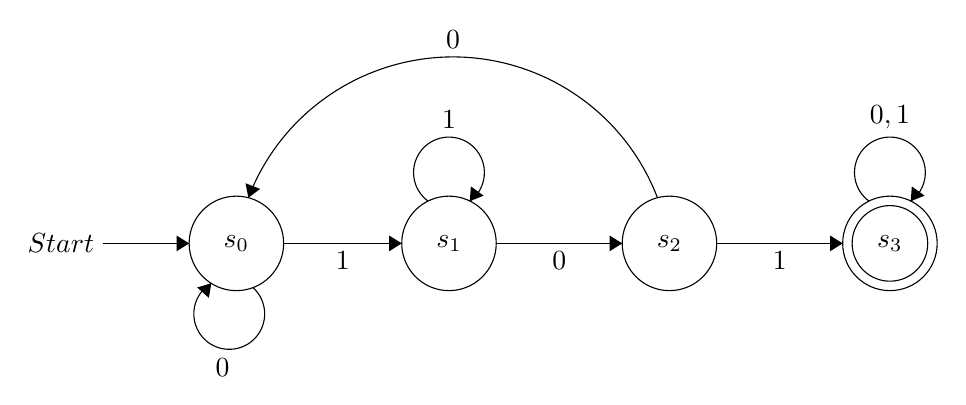
\begin{tikzpicture}[scale=0.2]
\tikzstyle{every node}+=[inner sep=0pt]
\draw [black] (17.8,-24.9) circle (3);
\draw (17.8,-24.9) node {$s_0$};
\draw [black] (31.3,-24.9) circle (3);
\draw (31.3,-24.9) node {$s_1$};
\draw [black] (45.3,-24.9) circle (3);
\draw (45.3,-24.9) node {$s_2$};
\draw [black] (59.3,-24.9) circle (3);
\draw (59.3,-24.9) node {$s_3$};
\draw [black] (59.3,-24.9) circle (2.4);
\draw [black] (9.3,-24.9) -- (14.8,-24.9);
\draw (8.8,-24.9) node [left] {$Start$};
\fill [black] (14.8,-24.9) -- (14,-24.4) -- (14,-25.4);
\draw [black] (20.8,-24.9) -- (28.3,-24.9);
\fill [black] (28.3,-24.9) -- (27.5,-24.4) -- (27.5,-25.4);
\draw (24.55,-25.4) node [below] {$1$};
\draw [black] (48.3,-24.9) -- (56.3,-24.9);
\fill [black] (56.3,-24.9) -- (55.5,-24.4) -- (55.5,-25.4);
\draw (52.3,-25.4) node [below] {$1$};
\draw [black] (57.977,-22.22) arc (234:-54:2.25);
\draw (59.3,-17.65) node [above] {$0,1$};
\fill [black] (60.62,-22.22) -- (61.5,-21.87) -- (60.69,-21.28);
\draw [black] (34.3,-24.9) -- (42.3,-24.9);
\fill [black] (42.3,-24.9) -- (41.5,-24.4) -- (41.5,-25.4);
\draw (38.3,-25.4) node [below] {$0$};
\draw [black] (18.845,-27.7) arc (48.19934:-239.80066:2.25);
\draw (16.92,-32.2) node [below] {$0$};
\fill [black] (16.21,-27.43) -- (15.31,-27.7) -- (16.05,-28.36);
\draw [black] (18.561,-22.004) arc (159.08853:20.91147:13.905);
\fill [black] (18.56,-22) -- (19.31,-21.44) -- (18.38,-21.08);
\draw (31.55,-12.56) node [above] {$0$};
\draw [black] (29.977,-22.22) arc (234:-54:2.25);
\draw (31.3,-17.65) node [above] {$1$};
\fill [black] (32.62,-22.22) -- (33.5,-21.87) -- (32.69,-21.28);
\end{tikzpicture}
\end{center}

\end{document}
